\documentclass[12pt,a4paper,twoside]{report}
\usepackage[utf8]{inputenc}
\usepackage[english]{babel}
\usepackage{indentfirst}
% \usepackage{enumitem}
% \usepackage{pdfpages}


\usepackage{listings}
\usepackage{color}

\usepackage{graphicx}
\graphicspath{ {./images/} }

\usepackage{cite}
\usepackage{hyperref}
\hypersetup{
	colorlinks=false,
	linkcolor=blue,
	filecolor=magenta,
	urlcolor=cyan,
}

\title{Master's thesis}
\author{Tomáš Belluš}

\definecolor{codegreen}{rgb}{0,0.6,0}
\definecolor{codegray}{rgb}{0.5,0.5,0.5}
\definecolor{codepurple}{rgb}{0.58,0,0.82}
\definecolor{backcolor}{rgb}{0.95,0.95,0.95}

\lstdefinestyle{codestyle}{
	commentstyle=\color{blue},
	keywordstyle=\color{black},
	numberstyle=\tiny\color{codegray},
	stringstyle=\color{codepurple},
	showstringspaces=false,
	captionpos=b,
}
\lstset{style=codestyle}

\lstdefinestyle{appendix}{
	basicstyle=\small\ttfamily,
	showstringspaces=false,
	captionpos=b,
	numbers=left,
	stepnumber=1,
	numberstyle=\small,
	breaklines=true,
}

\usepackage[utf8]{inputenc}
\usepackage[T1]{fontenc}
\usepackage[english]{babel}
\usepackage[a4paper]{geometry}
\usepackage[
    left = \glqq,% 
    right = \grqq,% 
    leftsub = \glq,% 
    rightsub = \grq%
]{dirtytalk}

% SETTINGS - NAMES
\newcommand{\myTitle}[0] {Bait network based monitoring of malicious actors}
\newcommand{\myName}[0] {Tomáš Belluš}
\newcommand{\mySupervisor}[0] {Ing. Tibor Csóka, PhD.}
\newcommand{\myEvidenceNumber}[0] {FIIT-XXXXXX-82385}
\newcommand{\myDate}[0] {May 2020}
\newcommand{\myStudyProgram}[0] {Information Security}
\newcommand{\myStudyField}[0] {9.2.4 Computer Engineering}
\newcommand{\myInstitude}[0] {Institute of Computer Engineering and Applied Informatics}

\usepackage[parfill]{parskip}
\usepackage{enumitem}

\usepackage{graphicx}
\usepackage{float}
\usepackage{longtable}
\usepackage{setspace}

% Spacing
\setstretch{\mySpacing}

\setcounter{secnumdepth}{3}
\setcounter{tocdepth}{3}

\usepackage{tabularx}
\newsavebox\mybox
\usepackage{fancyhdr}
\pagestyle{fancy}
\lhead{\nouppercase{\leftmark}}
\chead{}
\rhead{}
\lfoot{}
\cfoot{\thepage}
\rfoot{}


%style=iso-numeric
%style=authortitle-dw
\usepackage[maxnames=1,backend=bibtex,defernums=true]{biblatex}
\defbibheading{references}[Literature]{ 
  \chapter*{#1}
  \markboth{#1}{#1}
}
%\defbibheading{referencessec}[Literature]{ 
%  \section*{#1}
%  \markboth{#1}{#1}
%}
\bibliography{\myBibliography}


% Listing as figure
%\usepackage{libs/minted}
%\usepackage[section]{minted}

\usepackage{listing}

% openright does not work :(
\let\tmp\oddsidemargin
\let\oddsidemargin\evensidemargin
\let\evensidemargin\tmp
\reversemarginpar

\usepackage{lscape}
\usepackage{afterpage}

\usepackage{lipsum}
\usepackage{hyperref}

\begin{document}
	
%title page
\begin{center}
\thispagestyle{empty}
{\Large Slovak University of Technology in Bratislava}
\par\end{center}{\Large \par}

\begin{center}
{\Large Faculty of Informatics and Information Technologies}
\par\end{center}{\Large \par}

\smallskip{}

\begin{center}
\myEvidenceNumber
\par\end{center}
\vfill{}

\begin{center}
\textbf{\Large \myName}
\par\end{center}{\Large \par}

\medskip{}


\begin{center}
\textbf{\LARGE \myTitle }
\par\end{center}{\huge \par}

\medskip{}


\begin{center}

{\Large Výskumný zámer}
\par\end{center}{\Large \par}

\vfill{}

\noindent
Study program: \myStudyProgram

\noindent
Field of study: \myStudyField

\noindent
Training workplace: \myInstitude

\noindent
Supervisor: \mySupervisor

\medskip{}

\noindent
\myDate


\newpage
\thispagestyle{empty}
\mbox{}
\newpage



%assignment
\thispagestyle{empty}

% TODO: must be included !!!
% 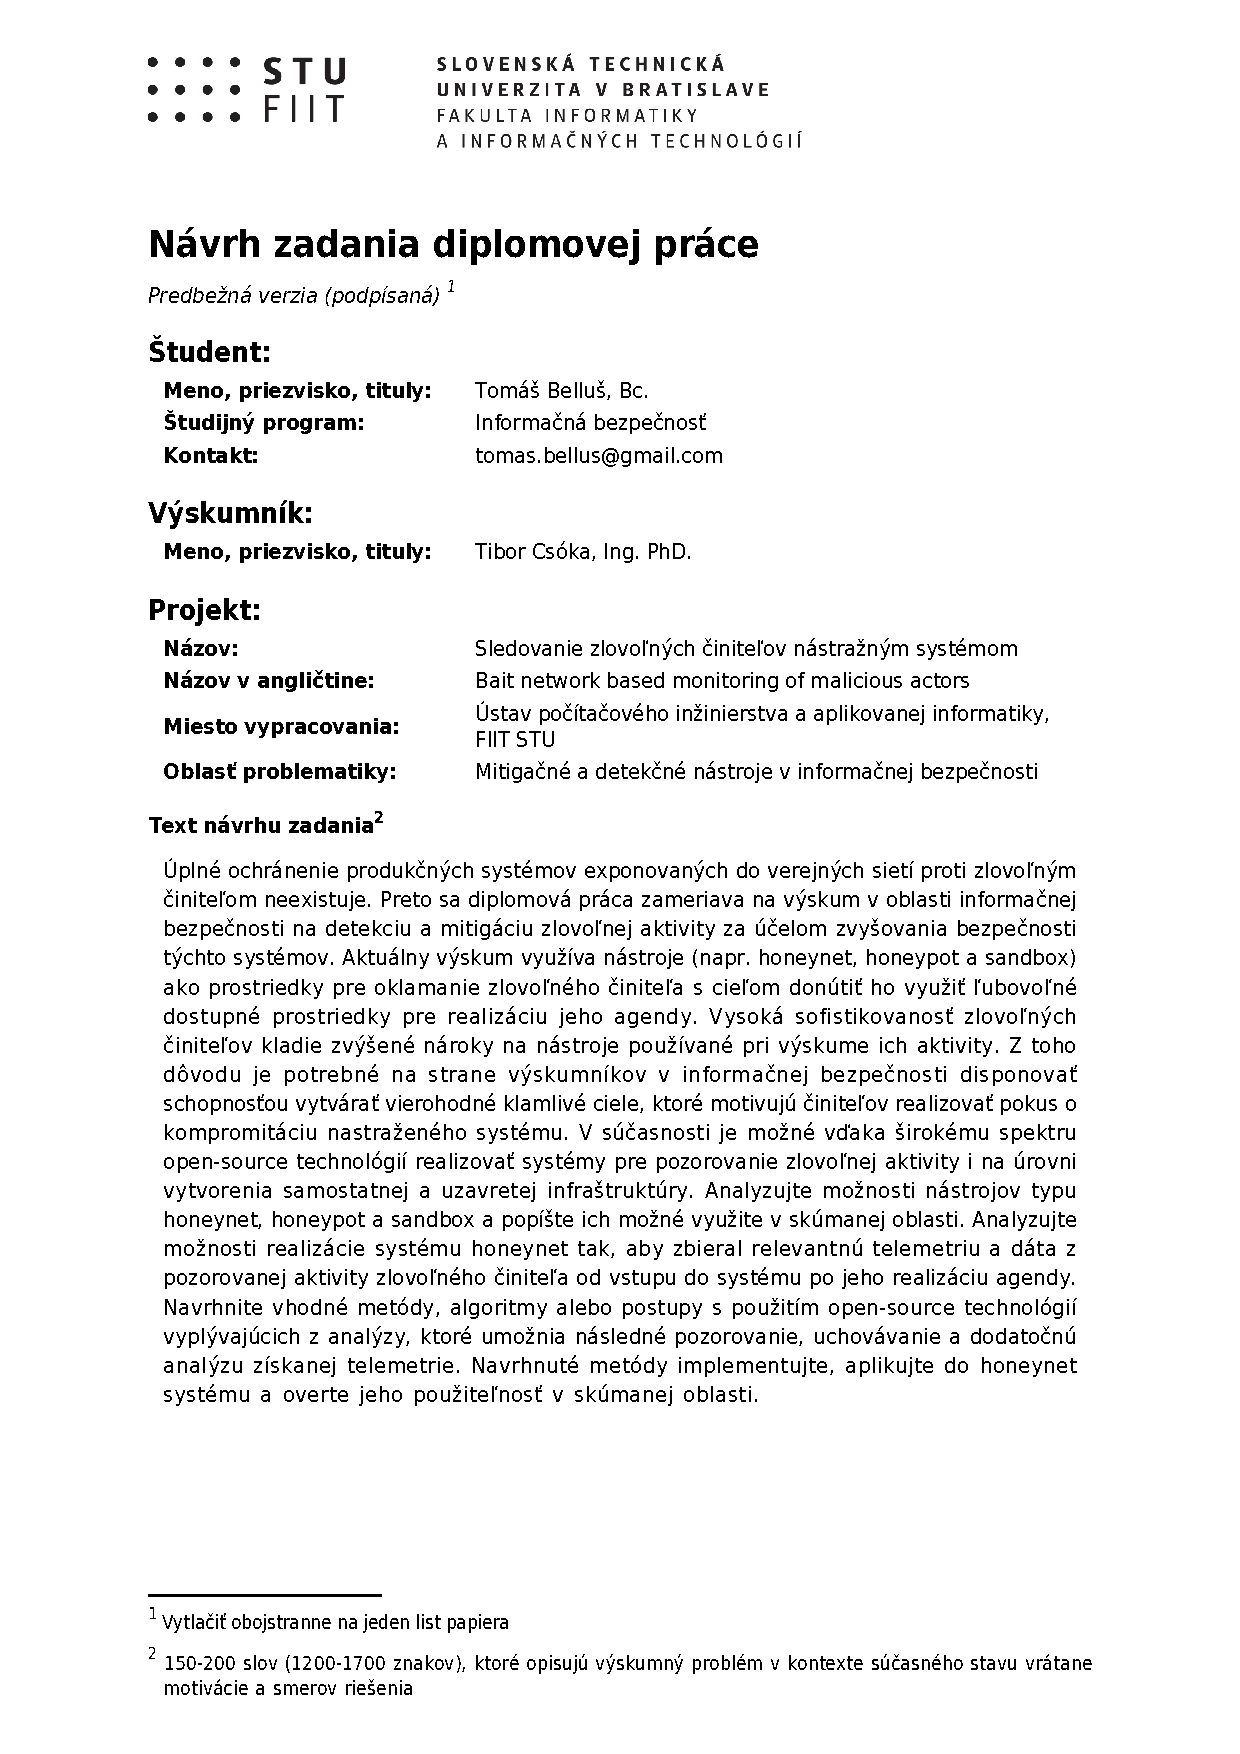
\includepdf[pages=-]{preamble/dp_zadanie.pdf}

\newpage{}\thispagestyle{empty}

\newpage
\thispagestyle{empty}
\mbox{}
\newpage

% table of contents
\begingroup
\color{black}
\tableofcontents
\endgroup


\chapter{Motivation}\label{motivation}

How to successfully delivery, exploit and compromise a target system?
Cyber criminals (attackers) follow a multi-phase process to completely
plan the sophisticated attack. The phases fall under so called
Cyber/Intrusion Kill Chain and include - reconnaissance, weaponization,
delivery, exploitation, installation, command and control, actions on objective
\footnote{\url{https://maritime-executive.com/blog/the-seven-phases-of-a-cyber-attack}}.
Briefly, the attack begins with analyzing and discovering the target
objective, followed by preparation of the exploit to compromise the
system and getting required control to fulfill a goal.

In contrast to the attackers, security experts use equally complex and
useful tools and practices to detect, mitigate or reproduce an attack.
Tools like sandbox, sinkhole, honeypot and many active detection tools
(e.g.~WAF, IPS/IDS, FW, etc.) In the "fight" of blue versus red, the
blue team must keep up with the red teams' techniques and zero-day
exploitation. Zero-day exploitation, or attack, target vulnerabilities
not addressed by vendors and not publicly known (beside the attackers)
\footnote{\url{https://us.norton.com/internetsecurity-emerging-threats-how-do-zero-day-vulnerabilities-work-30sectech.html}}.Such
vulnerabilities are almost impossible to mitigate and very difficult to
detect. White hat or ethical hackers search for these vulnerabilities in
their own environments by reading all those lines of code or dynamically
- utilizing honeypots.

Detecting zero-day vulnerabilities in a honeypot may result in a
absolute failure of the honeypot. The immutable infrastructure paradigm
would ensure the whole environment may be recovered. Usage of immutable
infrastructure may introduce the possibility of designing a complex
honeynet composed of multiple interconnected network segments and
devices.

\chapter{Analysis}\label{analysis}

"The primary technology that makes immutable infrastructure possible at
any scale is virtualization (both software and hardware) across
networking, servers, and storage"
\footnote{\url{https://www.sumologic.com/insight/mutable-immutable-infrastructure/}}.
According to this, virtualization is the inseparable element of
immutable infrastructure.

\subsection{Immutable infrastructure and its orchestration}\label{immutable-infrastructure-and-its-orchestration}

To understand the applications of immutable infrastructure one must
identify its characteristics. Any system or unit of a system
(i.e. container, VM, server) is pre-configured and deployed to its final
state in a target environment. The state is immutable - it forbids any
further configuration changes or additional networking. Required changes
are applied in the ``infrastructure configuration'' (e.g.~container
images) and redeployed to apply the updated state. In comparison, a
mutable infrastructure is the exact opposite, such as almost every
computer, that requires manual step-by-step installation of the OS and
the underlying applications and network configurations.

Having a complex infrastructure composed of multiple servers/containers
(any solo-standing service) allows segmentation of immutable services.
Instead of upgrading/modifying a whole infrastructure, only the desired
segments are addressed. Although, it introduces a problem of
orchestration and segmentation of services to the smallest unit
(i.e. container). Possible segmentation of services is discussed in the
next section - Escape attack mitigation. Orchestration is the question
of how, when and what combined in a single process of the mechanism
used.

The immutability has a profound effect on the security of the
infrastructure. Since every change is made by redeploying the
infrastructure, all ongoing attacks vanish despite being as complex as
outlast a reboot. \textbf{Although, the data stores (i.e.~databases,
message queues) are very much mutable components of the infrastructure,
therefore they should be subject to analysis.}

\subsection{Escape attack mitigation}\label{escape-attack-mitigation}

Escape attacks exploit vulnerabilities in shared resources or stack
level (e.g.~kernel for KVM, application for functions or hardware for
virtualization). A case study, with a goal to mitigate any form of
escape attacks, at the Swedish Police Authority by Christian Abdelmassih
-
\href{https://medium.com/@chrismessiah/docker-and-kubernetes-in-high-security-environments-d851645e8b99}{Docker
and Kubernetes in high security environments}. The author discusses
application isolation techniques while providing orchestration with
Kubernetes.

One technique is to isolate applications by containerization
(e.g.~Docker, LXC, etc.), which share the host's kernel. Second
technique is separation by bare-metal hypervisor - virtual machines
(VM). This means that the VM has it's own operation system (OS) and
shares hardware resources of the host. In conclusion, the idea is to
utilize bare-metal hypervisor (cloud native) to minimize the attack
surface for escape attacks, because containers are vulnerable to kernel
driven escape attacks.

To separate non-related application and utilize containers, he suggests
segmentation of Kubernetes pods to logical classes (e.i. class O, class
P and class PG). These classes are to be organized and orchestrated by
Kubernetes and should make sure nodes and pods have the same class tags.
Although, the solution was but present and lacks verification which
opens opportunities for my thesis, as the the author finalizes that ``In
order to utilize this in clouds in a scalable manner, there are
additional requirements for automation that must be satisfied. For
example, automating the creation of virtual machines, attaching them to
the Kubernetes cluster. Most importantly one must also implement and
verify that the application classifications are respected at all
times.'' {[}Chistian Abdelmassih, 24.01.2019{]}

\subsection{Honeypots \& Sandboxes}\label{honeypots-sandboxes}

Both honeypots and sandboxes are similarly used in dynamic threat
analysis. Difference is in preparation and isolation. Honeypot monitors
the activity of an attacker or a malware in emulated or production-like
environment. Sandbox is an isolated environment for dynamic malware
analysis with all preparation that is needed based on the knowledge of
the malware. Usually, honeypots are configured to detect specific
attacks with emulated applications or not emulated to detect zero-day
vulnerabilities and monitor behavior of potential exploitations
\footnote{\url{https://www.enisa.europa.eu/publications/proactive-detection-of-security-incidents-II-honeypots}}.
Within a sandbox, all activity is monitored as much as possible, while
knowing the outcome of the attack, to know the source of the attack.

A particularly interesting topic is to detect zero-day vulnerabilities
in a honeypot and, if necessary, replicating and more in depth analyzing
the exploitation in a sandbox. Analyzing malware in a sandbox provides
virtualization, which mitigates MBR overwrite. On the other hand, most
malwares verify the environment they're in - detection of virtualization
or sandbox awareness.

\chapter{Master's thesis overview}\label{masters-thesis-overview}

\section{Research questions}\label{research-questions}

How to improve virtualization/emulation detection in a honeypot or a
sandbox?

What is the most detectable phase in the Cyber Kill Chain?

The underlying technology for virtualization and containerization (if
any) is crucial to reach immutability. What provisioning and
orchestration mechanisms are needed to ensure an immutable
infrastructure?

\subsection{Thesis goal}\label{thesis-goal}

Design a honeypot or a sandbox, in Linux, as a dynamic analytic tool
dedicated to detect zero-day vulnerabilities and mitigating detection.
Utilize the immutable infrastructure paradigm to ensure automated and a
secure system. Mitigating escape attacks will not be in scope of this
thesis, but the introduced segmentation technique will be taken into
account to segregate related services.

\subsection{Plan of work}\label{plan-of-work}

\subsubsection{DP I}\label{dp-i}

\begin{itemize}
\item
  analyze virtualization (e.g KVM), emulation and virtualization
  detection mitigation practices
\item
  analyze cross-platform orchestration and provisioning mechanisms
\item
  comparison of existing solutions and discussion of possible
  improvements
\item
  design of ensuring immutability and the whole stack of the system
  supported by analysis
\end{itemize}

\subsubsection{DP II}\label{dp-ii}

\begin{itemize}
\item
  discuss possible attack vectors meant for monitoring
\item
  implementation of the system skeleton and configuration of the
  orchestartion mechanism

  \begin{itemize}
  \item
    create base images for the system
  \item
    automated deployment
  \end{itemize}
\item
  document the implementation
\item
  assignment revision of necessary
\end{itemize}

\subsubsection{DP III}\label{dp-iii}

\begin{itemize}
\item
  test honeypot implementation on live server
\item
  analyze all retrieved data and indicators of compromise
\item
  apply required modifications to images or core functionality
\item
  finalize the thesis documentation and evaluate reached goals
\end{itemize}

\chapter{Further Literature}\label{further-literature}

\url{https://pdfs.semanticscholar.org/d4e4/5e81b8d8878ca99648c3fc890ede1ae01b49.pdf}

\url{https://kth.diva-portal.org/smash/get/diva2:1231856/FULLTEXT02.pdf}

\url{https://www.enisa.europa.eu/publications/proactive-detection-of-security-incidents-II-honeypots}

\url{https://www.sumologic.com/insight/mutable-immutable-infrastructure/}

\end{document}